\documentclass{article}\usepackage[]{graphicx}\usepackage[]{color}
% maxwidth is the original width if it is less than linewidth
% otherwise use linewidth (to make sure the graphics do not exceed the margin)
\makeatletter
\def\maxwidth{ %
  \ifdim\Gin@nat@width>\linewidth
    \linewidth
  \else
    \Gin@nat@width
  \fi
}
\makeatother

\definecolor{fgcolor}{rgb}{0.345, 0.345, 0.345}
\newcommand{\hlnum}[1]{\textcolor[rgb]{0.686,0.059,0.569}{#1}}%
\newcommand{\hlstr}[1]{\textcolor[rgb]{0.192,0.494,0.8}{#1}}%
\newcommand{\hlcom}[1]{\textcolor[rgb]{0.678,0.584,0.686}{\textit{#1}}}%
\newcommand{\hlopt}[1]{\textcolor[rgb]{0,0,0}{#1}}%
\newcommand{\hlstd}[1]{\textcolor[rgb]{0.345,0.345,0.345}{#1}}%
\newcommand{\hlkwa}[1]{\textcolor[rgb]{0.161,0.373,0.58}{\textbf{#1}}}%
\newcommand{\hlkwb}[1]{\textcolor[rgb]{0.69,0.353,0.396}{#1}}%
\newcommand{\hlkwc}[1]{\textcolor[rgb]{0.333,0.667,0.333}{#1}}%
\newcommand{\hlkwd}[1]{\textcolor[rgb]{0.737,0.353,0.396}{\textbf{#1}}}%
\let\hlipl\hlkwb

\usepackage{framed}
\makeatletter
\newenvironment{kframe}{%
 \def\at@end@of@kframe{}%
 \ifinner\ifhmode%
  \def\at@end@of@kframe{\end{minipage}}%
  \begin{minipage}{\columnwidth}%
 \fi\fi%
 \def\FrameCommand##1{\hskip\@totalleftmargin \hskip-\fboxsep
 \colorbox{shadecolor}{##1}\hskip-\fboxsep
     % There is no \\@totalrightmargin, so:
     \hskip-\linewidth \hskip-\@totalleftmargin \hskip\columnwidth}%
 \MakeFramed {\advance\hsize-\width
   \@totalleftmargin\z@ \linewidth\hsize
   \@setminipage}}%
 {\par\unskip\endMakeFramed%
 \at@end@of@kframe}
\makeatother

\definecolor{shadecolor}{rgb}{.97, .97, .97}
\definecolor{messagecolor}{rgb}{0, 0, 0}
\definecolor{warningcolor}{rgb}{1, 0, 1}
\definecolor{errorcolor}{rgb}{1, 0, 0}
\newenvironment{knitrout}{}{} % an empty environment to be redefined in TeX

\usepackage{alltt}
\usepackage{amsmath} %This allows me to use the align functionality.
                     %If you find yourself trying to replicate
                     %something you found online, ensure you're
                     %loading the necessary packages!
\usepackage{amsfonts}%Math font
\usepackage{graphicx}%For including graphics
\usepackage{hyperref}%For Hyperlinks
\hypersetup{colorlinks = true,citecolor=black}
\usepackage{natbib}        %For the bibliography
\bibliographystyle{apalike}%For the bibliography
\usepackage[margin=0.5in]{geometry}
\usepackage{float}
\IfFileExists{upquote.sty}{\usepackage{upquote}}{}
\begin{document}
\noindent \textbf{MA 354: Data Analysis -- Fall 2021 -- Due 10/8 at 5p}\\%\\ gives you a new line
\noindent \textbf{Homework 2:}\vspace{1em}\\
\emph{Complete the following opportunities to use what we've talked about in class. These questions will be graded for correctness, communication and succinctness. Ensure you show your work and explain your logic in a legible and refined submission.}\\\vspace{1em}
%Comments -- anything after % is not put into the PDF

The starting jobs will be applied in alphabetical order (last name) for question two.
\begin{enumerate}
  \item \textbf{Solver:} provide a solution, if possible, and reasoning for the solution. \textbf{Due to group 10/5 or earlier.}
  \item \textbf{Code Checker:} provides a first check of the solver's worked solutions and ensures they are correct with a solid interpretation. 
  \item \textbf{Checker} checks the solution for completeness, proposes and implements changes if agreed upon by the group. Provides a short paragraph summarizing the discussion of proposals and their reason for acceptance or non-acceptance.
  \item \textbf{Double Checker} checks the solution for completeness, communication and polish. The Double Checker ensures that the solution is correct and highly polished for submission.
\end{enumerate}

\noindent For subsequent questions student roles will move down one position. The rolls change as follows.
\begin{enumerate}
  \item \textbf{Solver} $\Longrightarrow$ \textbf{Code Checker}
  \item \textbf{Code Checker} $\Longrightarrow$ \textbf{Checker}
  \item \textbf{Checker} $\Longrightarrow$ \textbf{Double Checker}
  \item \textbf{Double Checker} $\Longrightarrow$ \textbf{Solver}
\end{enumerate}
While students have assigned jobs for each question I encourage students to help 
each other complete the homework in collaboration.
\newpage
\begin{enumerate}
%%%%%%%%%%%%%%%%%%%%%%%%%%%%%%%%%%%%%%%%%%%%%%%%%%%%%%%%%%%%%%%%%%%%%%%%%%%%%%%%%%%%%%%%%%%
%%%%%%%%%%%%%%%%%%%%%%%%%%%%%%%%%%%%%%%%%%%%%%%%%%%%%%%%%%%%%%%%%%%%%%%%%%%%%%%%%%%%%%%%%%%
%%%%%%%%%  Question 1
%%%%%%%%%%%%%%%%%%%%%%%%%%%%%%%%%%%%%%%%%%%%%%%%%%%%%%%%%%%%%%%%%%%%%%%%%%%%%%%%%%%%%%%%%%%
%%%%%%%%%%%%%%%%%%%%%%%%%%%%%%%%%%%%%%%%%%%%%%%%%%%%%%%%%%%%%%%%%%%%%%%%%%%%%%%%%%%%%%%%%%%
  \item\label{Q1} Select a continuous distribution (Not the uniform or exponential). 
  It does not have to be one that we cover in the notes! To explore the PDF of your 
  distribution, specify two sets of parameter(s) for your distribution.
  \begin{enumerate}
  %%%%%%%%%%%%%%%%%%%%%%%%%%%%%%%%%%%%%%%%%%%%%%%%%%%%%%%%%%%%%%%%%%%%%%%%%%%%%%%%%%%%%%%%%%%
  %%%%%%%%%  Part (a)
  %%%%%%%%%%%%%%%%%%%%%%%%%%%%%%%%%%%%%%%%%%%%%%%%%%%%%%%%%%%%%%%%%%%%%%%%%%%%%%%%%%%%%%%%%%%
  \item \textbf{History} Discuss what types of random variables are modeled with 
  your distribution. Be sure to include a discussion about the support and ensure 
  to provide the density function, and CDF. This requires some internet research 
  -- what's the history of the distribution, why was it created and named? What 
  are some exciting applications of this distribution?
  
  Cite all of your sources in LaTeX by adding a BibTeX citation to the .bib file. 
  To help, I've cited R \citep{R21} in parentheses here. \cite{R21} provides helpful 
  tools for the rest of the questions below. BibTeX citations are available through 
  Google Scholar by clicking the cite button below the article of  interest and 
  selecting the BibTeX option.\\
  
  \textbf{Solution:}\\
  Our group has chosen to use a normal distribution for the \texttt{Q1} and \texttt{Q2}!\\
  To start with, I will define what a normal distribution is. A continuous variable X has a normal distribution — with mean $\mu$ and $\sigma^2$ — X ~ N($\mu, \sigma^2)$, if it has the following properties:\\
  		\begin{equation*}
	\mu \in \mathbb{R}; \sigma \in \mathbb{R}^+
	\tag{\textbf{Parameters}}
	\end{equation*}
	
	\begin{equation*}
	X = \{x:x\in\mathbb{R}\}
	\tag{\textbf{Support}}
	\end{equation*}
  	
  	\begin{equation*}
	f_{X}({x|\mu,\sigma})=\frac{1}{\sigma\sqrt{2\pi}}e^\frac{-(x-\mu)^2}{2\sigma^2} \tag{\textbf{PDF}}\\
	\end{equation*}
	
	\begin{equation*}
	F_{X}({x|\mu,\sigma})=\int_{-\infty}^{\infty}\frac{1}{\sigma\sqrt{2\pi}}e^\frac{-(x-\mu)^2}{2\sigma^2} \tag{\textbf{CDF}}
	\end{equation*}
  
  \textbf{Description:} Normal distribution is one of the most important distributions in the world of statistics, and it's used in many fields. The graph of this probability function is a symmetric, bell-shaped curved. Symmetry of this function implies that its mean is going to be equal to its median value. We are going to prove it later on. \\
  \textbf{History:} One of the first major great discoveries in the field of statistics happened in 1713, as Jacob Bernoulli published his work on proving the Weak Law of Large Numbers. According to \cite{patel1996handbook}, initially normal distribution appeared in 1733 as an approximation to the probability for sums of binominally distributed quantities to lie between two values. \\
  \textbf{Today:} According to \cite{ahsanullah2014normal}, normal distribution plays an important role in many applied problems in biology, economics, engineering, genetics, hydrology, mechanics, medicine, number theory, statistics, physics, psychology and so on. 
  
  
  %%%%%%%%%%%%%%%%%%%%%%%%%%%%%%%%%%%%%%%%%%%%%%%%%%%%%%%%%%%%%%%%%%%%%%%%%%%%%%%%%%%%%%%%%%%
  %%%%%%%%%  Part (b)
  %%%%%%%%%%%%%%%%%%%%%%%%%%%%%%%%%%%%%%%%%%%%%%%%%%%%%%%%%%%%%%%%%%%%%%%%%%%%%%%%%%%%%%%%%%%
	\item Show that you have a valid PDF. You will find the \texttt{integrate()} 
	function in \texttt{R} helpful.\\
	
	\textbf{Solution:}\\
	Here's the equation of PDF for normal distribution!
	\begin{equation*}
	f_{X}({x|\mu,\sigma})=\frac{1}{\sigma\sqrt{2\pi}}e^\frac{-(x-\mu)^2}{2\sigma^2} \tag{\textbf{PDF}}
	\end{equation*}
	Now, let's prove that it's valid!\\
	Since normal (or gaussian — whatever you prefer!) distribution is a continous probability distribution, it implies that the area under the curve is equal to 1 (or 100\%!). This statement takes its roots from the second Kolmogorov axiom that states that the entirety of sample space is equal to one.\\
	Therefore, let's use CDF to prove that our PDF formula is going to return one! Since the support for normal distribution contain all rational numbers, our integral is going to be from negative infinity to positive infinity. 
	\begin{equation*}
	F_{X}({x|\mu,\sigma})=\int_{-\infty}^{\infty}\frac{1}{\sigma\sqrt{2\pi}}e^\frac{-(x-\mu)^2}{2\sigma^2} \tag{\textbf{CDF}}
	\end{equation*}
	I am going to use \texttt{integrate()} function in order to compute this equation.
\begin{knitrout}
\definecolor{shadecolor}{rgb}{0.969, 0.969, 0.969}\color{fgcolor}\begin{kframe}
\begin{alltt}
\hlstd{mean}\hlkwb{<-}\hlnum{1} \hlcom{#mu}
\hlstd{sd}\hlkwb{<-}\hlnum{3} \hlcom{#sigma}
\hlstd{pdf} \hlkwb{<-} \hlkwa{function}\hlstd{(}\hlkwc{x}\hlstd{)\{}
  \hlstd{(}\hlnum{1}\hlopt{/}\hlstd{(sd}\hlopt{*}\hlkwd{sqrt}\hlstd{(}\hlnum{2}\hlopt{*}\hlstd{pi)))}\hlopt{*}\hlkwd{exp}\hlstd{((}\hlopt{-}\hlstd{(x}\hlopt{-}\hlstd{mean)}\hlopt{^}\hlnum{2}\hlstd{)}\hlopt{/}\hlstd{(}\hlnum{2}\hlopt{*}\hlstd{sd}\hlopt{^}\hlnum{2}\hlstd{))} \hlcom{#our PDF}
\hlstd{\}}
\hlkwd{integrate}\hlstd{(pdf,} \hlopt{-}\hlnum{Inf}\hlstd{,} \hlnum{Inf}\hlstd{)} \hlcom{#CDF for total area under the curve}
\end{alltt}
\begin{verbatim}
## 1 with absolute error < 2.1e-07
\end{verbatim}
\end{kframe}
\end{knitrout}
	
	%%%%%%%%%%%%%%%%%%%%%%%%%%%%%%%%%%%%%%%%%%%%%%%%%%%%%%%%%%%%%%%%%%%%%%%%%%%%%%%%%%%%%%%%%%%
  %%%%%%%%%  Part (c)
  %%%%%%%%%%%%%%%%%%%%%%%%%%%%%%%%%%%%%%%%%%%%%%%%%%%%%%%%%%%%%%%%%%%%%%%%%%%%%%%%%%%%%%%%%%%
	\item Find the median for your two sets of parameter(s). Conduct some research 
	to find the median based on our PDF to confirm that your numerical approach is 
	correct. \\
	
	\textbf{Solution:}\\
	As we have established in part \texttt{(a)} of this problem, one of the key features of the normal distribution is the fact that it's symmetrical. Let's set out to prove it through the direct proof!\\
		Let \texttt{m} be median!
		\begin{equation*}
	P(X\le m)=P(X\ge m)=\frac{1}{2}
	\tag{\textbf{Definition of the median}}
	\end{equation*}
	Let normal distribution be symmetric. If it's symmetric, then the statement $\mu=m$ holds true.\\
	Therefore, the following equation should also hold true:
	\begin{equation*}
\int_{-\infty}^{\mu}\frac{1}{\sigma\sqrt{2\pi}}e^\frac{-(x-\mu)^2}{2\sigma^2}=
\int_{\mu}^{\infty}\frac{1}{\sigma\sqrt{2\pi}}e^\frac{-(x-\mu)^2}{2\sigma^2}=
\frac{1}{2}
\tag{\textbf{Assumption}}
	\end{equation*}
	
	Let's check it through R!
\begin{knitrout}
\definecolor{shadecolor}{rgb}{0.969, 0.969, 0.969}\color{fgcolor}\begin{kframe}
\begin{alltt}
        \hlstd{mean}\hlkwb{<-}\hlnum{1} \hlcom{#mu}
        \hlstd{sd}\hlkwb{<-}\hlnum{3} \hlcom{#sigma}
        \hlstd{func} \hlkwb{<-} \hlkwa{function}\hlstd{(}\hlkwc{x}\hlstd{)\{}
          \hlstd{(}\hlnum{1}\hlopt{/}\hlstd{(sd}\hlopt{*}\hlkwd{sqrt}\hlstd{(}\hlnum{2}\hlopt{*}\hlstd{pi)))}\hlopt{*}\hlkwd{exp}\hlstd{((}\hlopt{-}\hlstd{(x}\hlopt{-}\hlstd{mean)}\hlopt{^}\hlnum{2}\hlstd{)}\hlopt{/}\hlstd{(}\hlnum{2}\hlopt{*}\hlstd{sd}\hlopt{^}\hlnum{2}\hlstd{))}
        \hlstd{\}}
        \hlstd{firstPart} \hlkwb{<-} \hlkwd{integrate}\hlstd{(func,} \hlopt{-}\hlnum{Inf}\hlstd{, mean)}
        \hlstd{secondPart} \hlkwb{<-} \hlkwd{integrate}\hlstd{(func, mean,} \hlnum{Inf}\hlstd{)}

        \hlstd{(firstPart}\hlopt{$}\hlstd{value)}
\end{alltt}
\begin{verbatim}
## [1] 0.5
\end{verbatim}
\begin{alltt}
        \hlstd{(firstPart}\hlopt{$}\hlstd{value}\hlopt{==}\hlstd{secondPart}\hlopt{$}\hlstd{value)}
\end{alltt}
\begin{verbatim}
## [1] TRUE
\end{verbatim}
\end{kframe}
\end{knitrout}

It would appear that $\mu=m!$ Therefore, mean is equal to median within the normal distribution. Therefore, since $\mu_{1}=1$ and $\mu_{2}=-2$, the medians are 1 and -2 respectively!
	%%%%%%%%%%%%%%%%%%%%%%%%%%%%%%%%%%%%%%%%%%%%%%%%%%%%%%%%%%%%%%%%%%%%%%%%%%%%%%%%%%%%%%%%%%%
  %%%%%%%%%  Part (d)
  %%%%%%%%%%%%%%%%%%%%%%%%%%%%%%%%%%%%%%%%%%%%%%%%%%%%%%%%%%%%%%%%%%%%%%%%%%%%%%%%%%%%%%%%%%%
	\item \label{q1PDF} Graph the PDF for several values of the parameter(s) 
	including the two sets you specified. What does changing the parameter(s) do 
	to the shape of the PDF?\\
	
	\textbf{Solution:}\\
	Let's take various values and plot different PDFs! I am going to use  the ggplot2 \citep{ggplot2} library for it!
\begin{figure}[H]
\begin{center}
\begin{knitrout}
\definecolor{shadecolor}{rgb}{0.969, 0.969, 0.969}\color{fgcolor}\begin{kframe}
\begin{alltt}
\hlkwd{library}\hlstd{(ggplot2)}
\hlstd{plot.df} \hlkwb{<-} \hlkwd{data.frame}\hlstd{(}
  \hlkwc{x}\hlstd{=}\hlkwd{seq}\hlstd{(}\hlopt{-}\hlnum{15}\hlstd{,} \hlnum{15}\hlstd{,} \hlnum{0.001}\hlstd{),}
  \hlkwc{f1}\hlstd{=}\hlkwd{dnorm}\hlstd{(}\hlkwc{x}\hlstd{=}\hlkwd{seq}\hlstd{(}\hlopt{-}\hlnum{15}\hlstd{,} \hlnum{15}\hlstd{,} \hlnum{0.001}\hlstd{),} \hlkwc{mean}\hlstd{=}\hlnum{1}\hlstd{,} \hlkwc{sd}\hlstd{=}\hlnum{1}\hlstd{),}
  \hlkwc{f2}\hlstd{=}\hlkwd{dnorm}\hlstd{(}\hlkwc{x}\hlstd{=}\hlkwd{seq}\hlstd{(}\hlopt{-}\hlnum{15}\hlstd{,} \hlnum{15}\hlstd{,} \hlnum{0.001}\hlstd{),} \hlkwc{mean}\hlstd{=}\hlopt{-}\hlnum{2}\hlstd{,} \hlkwc{sd}\hlstd{=}\hlnum{4}\hlstd{),}
  \hlkwc{f3}\hlstd{=}\hlkwd{dnorm}\hlstd{(}\hlkwc{x}\hlstd{=}\hlkwd{seq}\hlstd{(}\hlopt{-}\hlnum{15}\hlstd{,} \hlnum{15}\hlstd{,} \hlnum{0.001}\hlstd{),} \hlkwc{mean}\hlstd{=}\hlnum{0}\hlstd{,} \hlkwc{sd}\hlstd{=}\hlnum{5}\hlstd{),}
  \hlkwc{f4}\hlstd{=}\hlkwd{dnorm}\hlstd{(}\hlkwc{x}\hlstd{=}\hlkwd{seq}\hlstd{(}\hlopt{-}\hlnum{15}\hlstd{,} \hlnum{15}\hlstd{,} \hlnum{0.001}\hlstd{),} \hlkwc{mean}\hlstd{=}\hlnum{3}\hlstd{,} \hlkwc{sd}\hlstd{=}\hlnum{3}\hlstd{)}
\hlstd{)}

\hlkwd{ggplot}\hlstd{(plot.df,} \hlkwd{aes}\hlstd{(}\hlkwc{x}\hlstd{=x))}\hlopt{+}
  \hlkwd{geom_line}\hlstd{(}\hlkwd{aes}\hlstd{(}\hlkwc{y}\hlstd{=f1,} \hlkwc{color}\hlstd{=}\hlstr{"m=1, sd=1"}\hlstd{))}\hlopt{+}
  \hlkwd{geom_line}\hlstd{(}\hlkwd{aes}\hlstd{(}\hlkwc{y}\hlstd{=f2,} \hlkwc{color}\hlstd{=}\hlstr{"m=-2, sd=4"}\hlstd{))}\hlopt{+}
  \hlkwd{geom_line}\hlstd{(}\hlkwd{aes}\hlstd{(}\hlkwc{y}\hlstd{=f3,} \hlkwc{color}\hlstd{=}\hlstr{"m=0, sd=5"}\hlstd{))}\hlopt{+}
  \hlkwd{geom_line}\hlstd{(}\hlkwd{aes}\hlstd{(}\hlkwc{y}\hlstd{=f4,} \hlkwc{color}\hlstd{=}\hlstr{"m=3, sd=3"}\hlstd{))}\hlopt{+}
  \hlkwd{theme_bw}\hlstd{()}
\end{alltt}
\end{kframe}
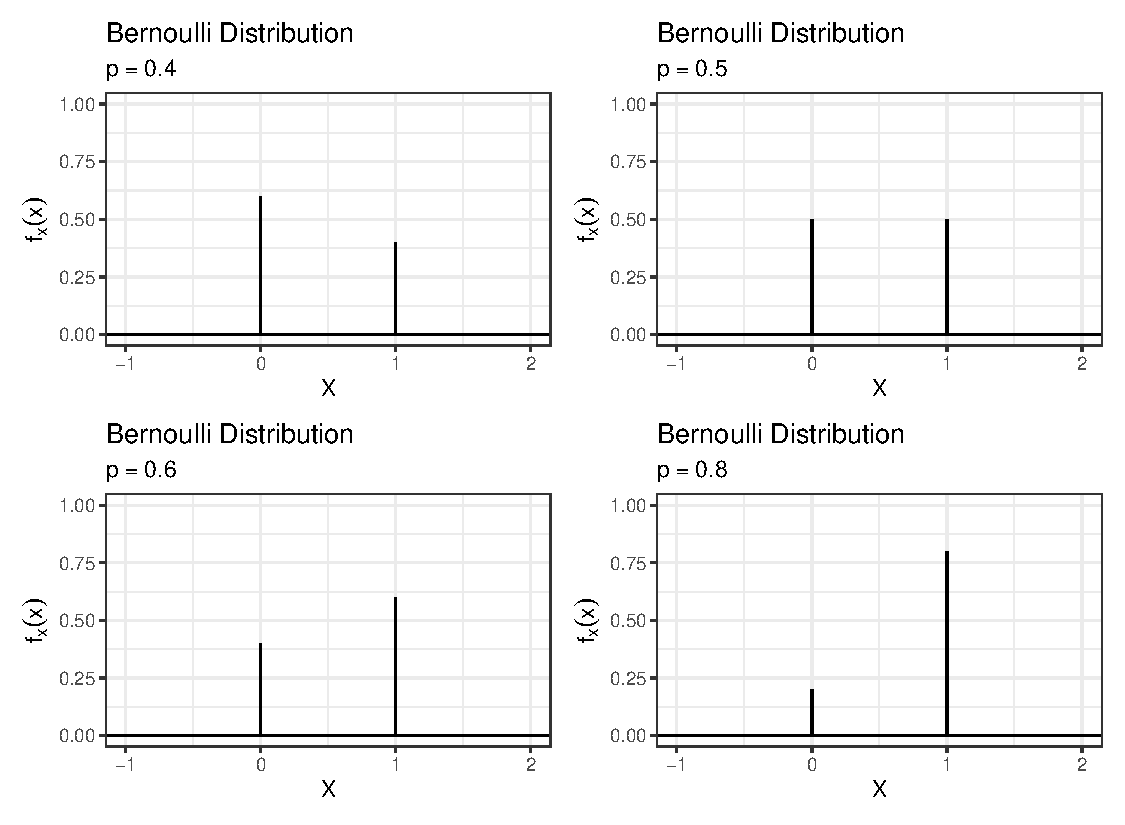
\includegraphics[width=\maxwidth]{figure/unnamed-chunk-3-1} 
\end{knitrout}
\caption{Gaussian PDF with various sets of parameters}
\label{plot1}
\end{center}
\end{figure}
As we can see on Figure \ref{plot1}, changing our parameters does indeed change the graph we have. Changing the $\mu$ transforms graph to the right (if the mean is positive) and to the left (if the mean is negative). Changing $\sigma$ changes the kurtosis of the graph. Thus, distributions with lower value of $\sigma$ show higher peaks.
	%%%%%%%%%%%%%%%%%%%%%%%%%%%%%%%%%%%%%%%%%%%%%%%%%%%%%%%%%%%%%%%%%%%%%%%%%%%%%%%%%%%%%%%%%%%
  %%%%%%%%%  Part (e)
  %%%%%%%%%%%%%%%%%%%%%%%%%%%%%%%%%%%%%%%%%%%%%%%%%%%%%%%%%%%%%%%%%%%%%%%%%%%%%%%%%%%%%%%%%%%
	 \item Graph the CDF for the same values of the parameter(s) as you did in 
	 Question \ref{q1PDF}. What does changing the parameter(s) do to the shape of 
	 the CDF? Comment on the aspects of the CDFs that show that the CDF is valid.\\
	 
	 \textbf{Solution:}\\
\begin{figure}[H]
\begin{center}
\begin{knitrout}
\definecolor{shadecolor}{rgb}{0.969, 0.969, 0.969}\color{fgcolor}\begin{kframe}
\begin{alltt}
\hlstd{plot.df} \hlkwb{<-} \hlkwd{data.frame}\hlstd{(}
  \hlkwc{x}\hlstd{=}\hlkwd{seq}\hlstd{(}\hlopt{-}\hlnum{15}\hlstd{,} \hlnum{15}\hlstd{,} \hlnum{0.001}\hlstd{),}
  \hlkwc{f1}\hlstd{=}\hlkwd{pnorm}\hlstd{(}\hlkwc{q}\hlstd{=}\hlkwd{seq}\hlstd{(}\hlopt{-}\hlnum{15}\hlstd{,} \hlnum{15}\hlstd{,} \hlnum{0.001}\hlstd{),} \hlkwc{mean}\hlstd{=}\hlnum{1}\hlstd{,} \hlkwc{sd}\hlstd{=}\hlnum{1}\hlstd{),}
  \hlkwc{f2}\hlstd{=}\hlkwd{pnorm}\hlstd{(}\hlkwc{q}\hlstd{=}\hlkwd{seq}\hlstd{(}\hlopt{-}\hlnum{15}\hlstd{,} \hlnum{15}\hlstd{,} \hlnum{0.001}\hlstd{),} \hlkwc{mean}\hlstd{=}\hlopt{-}\hlnum{2}\hlstd{,} \hlkwc{sd}\hlstd{=}\hlnum{4}\hlstd{),}
  \hlkwc{f3}\hlstd{=}\hlkwd{pnorm}\hlstd{(}\hlkwc{q}\hlstd{=}\hlkwd{seq}\hlstd{(}\hlopt{-}\hlnum{15}\hlstd{,} \hlnum{15}\hlstd{,} \hlnum{0.001}\hlstd{),} \hlkwc{mean}\hlstd{=}\hlnum{0}\hlstd{,} \hlkwc{sd}\hlstd{=}\hlnum{5}\hlstd{),}
  \hlkwc{f4}\hlstd{=}\hlkwd{pnorm}\hlstd{(}\hlkwc{q}\hlstd{=}\hlkwd{seq}\hlstd{(}\hlopt{-}\hlnum{15}\hlstd{,} \hlnum{15}\hlstd{,} \hlnum{0.001}\hlstd{),} \hlkwc{mean}\hlstd{=}\hlnum{3}\hlstd{,} \hlkwc{sd}\hlstd{=}\hlnum{3}\hlstd{)}
\hlstd{)}

\hlkwd{ggplot}\hlstd{(plot.df,} \hlkwd{aes}\hlstd{(}\hlkwc{x}\hlstd{=x))}\hlopt{+}
  \hlkwd{geom_line}\hlstd{(}\hlkwd{aes}\hlstd{(}\hlkwc{y}\hlstd{=f1,} \hlkwc{color}\hlstd{=}\hlstr{"m=1, sd=1"}\hlstd{))}\hlopt{+}
  \hlkwd{geom_line}\hlstd{(}\hlkwd{aes}\hlstd{(}\hlkwc{y}\hlstd{=f2,} \hlkwc{color}\hlstd{=}\hlstr{"m=-2, sd=4"}\hlstd{))}\hlopt{+}
  \hlkwd{geom_line}\hlstd{(}\hlkwd{aes}\hlstd{(}\hlkwc{y}\hlstd{=f3,} \hlkwc{color}\hlstd{=}\hlstr{"m=0, sd=5"}\hlstd{))}\hlopt{+}
  \hlkwd{geom_line}\hlstd{(}\hlkwd{aes}\hlstd{(}\hlkwc{y}\hlstd{=f4,} \hlkwc{color}\hlstd{=}\hlstr{"m=3, sd=3"}\hlstd{))}\hlopt{+}
  \hlkwd{theme_bw}\hlstd{()}
\end{alltt}
\end{kframe}
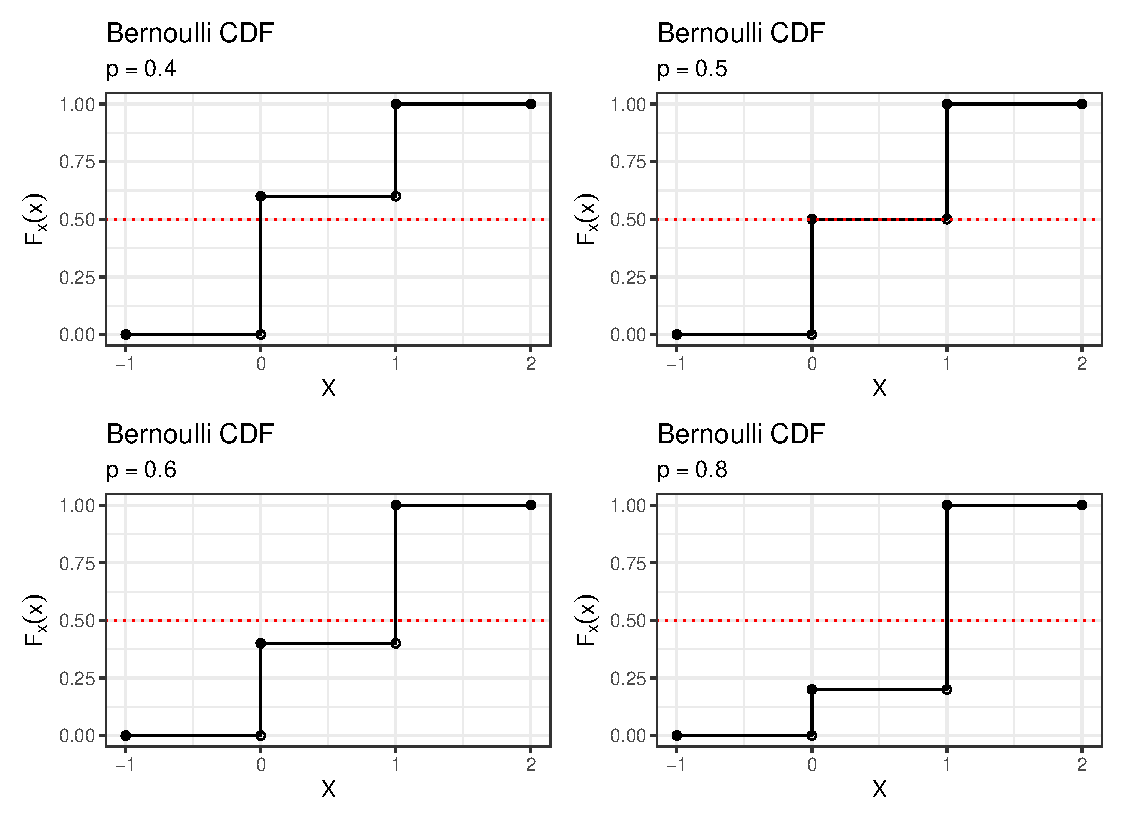
\includegraphics[width=\maxwidth]{figure/unnamed-chunk-4-1} 
\end{knitrout}

\caption{Gaussian CDF with various sets of parameters}
\label{plot2} %we can now reference plot1
\end{center}
\end{figure}

We see that Figure \ref{plot2} is a graph of CDF function with different sets of parameters. This function shows the probability that a probability that a random variable X will take a value less than or equal to $x$. We can see that our PDF is valid, for when we went over all values of X, the probability is $1.00$ or 100\%. Changing the value of $\mu$ changes the position of a graph (moves it to the right or to the left), while the change in $\sigma$ increases the slope of the function: the higher the value of $\sigma$, the faster the function will go over all the values and reach 100\%.
	%%%%%%%%%%%%%%%%%%%%%%%%%%%%%%%%%%%%%%%%%%%%%%%%%%%%%%%%%%%%%%%%%%%%%%%%%%%%%%%%%%%%%%%%%%%
  %%%%%%%%%  Part (f)
  %%%%%%%%%%%%%%%%%%%%%%%%%%%%%%%%%%%%%%%%%%%%%%%%%%%%%%%%%%%%%%%%%%%%%%%%%%%%%%%%%%%%%%%%%%%
  \item Generate a random sample of size $n=10, 25, 100$, and $1000$ for your 
  two sets of parameter(s). In a $4 \times 2$ grid, plot a histogram of each set
  of data and superimpose the true density function at the specified parameter 
  values. Interpret the results.\\
  
  \textbf{Solution:}\\

\begin{knitrout}
\definecolor{shadecolor}{rgb}{0.969, 0.969, 0.969}\color{fgcolor}\begin{kframe}
\begin{alltt}
        \hlkwd{library}\hlstd{(patchwork)}
        \hlkwd{library}\hlstd{(tidyverse)}

        \hlstd{sample.df} \hlkwb{<-} \hlkwd{list}\hlstd{(}\hlkwc{x1}\hlstd{=}\hlkwd{rnorm}\hlstd{(}\hlnum{10}\hlstd{,} \hlkwc{mean}\hlstd{=}\hlnum{1}\hlstd{,} \hlkwc{sd}\hlstd{=}\hlnum{1}\hlstd{),}
                               \hlkwc{x2}\hlstd{=}\hlkwd{rnorm}\hlstd{(}\hlnum{25}\hlstd{,} \hlkwc{mean}\hlstd{=}\hlnum{1}\hlstd{,} \hlkwc{sd}\hlstd{=}\hlnum{1}\hlstd{),}
                               \hlkwc{x3}\hlstd{=}\hlkwd{rnorm}\hlstd{(}\hlnum{100}\hlstd{,} \hlkwc{mean}\hlstd{=}\hlnum{1}\hlstd{,} \hlkwc{sd}\hlstd{=}\hlnum{1}\hlstd{),}
                               \hlkwc{x4}\hlstd{=}\hlkwd{rnorm}\hlstd{(}\hlnum{1000}\hlstd{,} \hlkwc{mean}\hlstd{=}\hlnum{1}\hlstd{,} \hlkwc{sd}\hlstd{=}\hlnum{1}\hlstd{),}
                               \hlkwc{y1}\hlstd{=}\hlkwd{rnorm}\hlstd{(}\hlnum{10}\hlstd{,} \hlkwc{mean}\hlstd{=}\hlopt{-}\hlnum{2}\hlstd{,} \hlkwc{sd}\hlstd{=}\hlnum{4}\hlstd{),}
                               \hlkwc{y2}\hlstd{=}\hlkwd{rnorm}\hlstd{(}\hlnum{25}\hlstd{,} \hlkwc{mean}\hlstd{=}\hlopt{-}\hlnum{2}\hlstd{,} \hlkwc{sd}\hlstd{=}\hlnum{4}\hlstd{),}
                               \hlkwc{y3}\hlstd{=}\hlkwd{rnorm}\hlstd{(}\hlnum{100}\hlstd{,} \hlkwc{mean}\hlstd{=}\hlopt{-}\hlnum{2}\hlstd{,} \hlkwc{sd}\hlstd{=}\hlnum{4}\hlstd{),}
                               \hlkwc{y4}\hlstd{=}\hlkwd{rnorm}\hlstd{(}\hlnum{1000}\hlstd{,} \hlkwc{mean}\hlstd{=}\hlopt{-}\hlnum{2}\hlstd{,} \hlkwc{sd}\hlstd{=}\hlnum{4}\hlstd{))}

        \hlstd{buildingPlot} \hlkwb{<-} \hlkwa{function}\hlstd{(}\hlkwc{source}\hlstd{,} \hlkwc{mu}\hlstd{,} \hlkwc{sigma}\hlstd{)\{}
          \hlstd{df} \hlkwb{<-} \hlkwd{data.frame}\hlstd{(}\hlkwc{value}\hlstd{=source)} \hlcom{#turning values from the list into a df}
          \hlkwd{colnames}\hlstd{(df)} \hlkwb{<-} \hlstr{"value"} \hlcom{#changing the name of the column}

          \hlstd{answer}\hlkwb{<-}\hlkwd{ggplot}\hlstd{(df,} \hlkwd{aes}\hlstd{(value))}\hlopt{+}
            \hlkwd{geom_histogram}\hlstd{(}\hlkwd{aes}\hlstd{(}\hlkwc{y}\hlstd{=..density..),} \hlkwc{bins}\hlstd{=}\hlnum{10}\hlstd{,}
                         \hlkwc{color}\hlstd{=}\hlstr{"black"}\hlstd{)}\hlopt{+} \hlcom{#building a histogram}
            \hlkwd{geom_function}\hlstd{(}\hlkwc{fun}\hlstd{=dnorm,} \hlkwc{args} \hlstd{=} \hlkwd{list}\hlstd{(}\hlkwc{mean} \hlstd{= mu,} \hlkwc{sd} \hlstd{= sigma),}
                \hlkwc{color}\hlstd{=}\hlstr{"red"}\hlstd{)}\hlopt{+}
            \hlkwd{theme_bw}\hlstd{()} \hlopt{+}\hlcom{#superimposing the function}
            \hlkwd{labs}\hlstd{(}\hlkwc{x}\hlstd{=}\hlstr{"Value"}\hlstd{,} \hlkwc{y}\hlstd{=}\hlstr{"Density"}\hlstd{)}
          \hlstd{answer}
        \hlstd{\}}

        \hlstd{x1}\hlkwb{<-}\hlkwd{buildingPlot}\hlstd{(sample.df[}\hlnum{1}\hlstd{],} \hlnum{1}\hlstd{,} \hlnum{1}\hlstd{)}\hlopt{+}\hlkwd{labs}\hlstd{(}\hlkwc{title}\hlstd{=}\hlstr{"Sample=10"}\hlstd{,}
                                                  \hlkwc{subtitle} \hlstd{=} \hlstr{"mean=1, sd=1"}\hlstd{)}
        \hlstd{x2}\hlkwb{<-}\hlkwd{buildingPlot}\hlstd{(sample.df[}\hlnum{2}\hlstd{],} \hlnum{1}\hlstd{,} \hlnum{1}\hlstd{)}\hlopt{+}\hlkwd{labs}\hlstd{(}\hlkwc{title}\hlstd{=}\hlstr{"Sample=25"}\hlstd{,}
                                                  \hlkwc{subtitle} \hlstd{=} \hlstr{"mean=1, sd=1"}\hlstd{)}
        \hlstd{x3}\hlkwb{<-}\hlkwd{buildingPlot}\hlstd{(sample.df[}\hlnum{3}\hlstd{],} \hlnum{1}\hlstd{,} \hlnum{1}\hlstd{)}\hlopt{+}\hlkwd{labs}\hlstd{(}\hlkwc{title}\hlstd{=}\hlstr{"Sample=100"}\hlstd{,}
                                                  \hlkwc{subtitle} \hlstd{=} \hlstr{"mean=1, sd=1"}\hlstd{)}
        \hlstd{x4}\hlkwb{<-}\hlkwd{buildingPlot}\hlstd{(sample.df[}\hlnum{4}\hlstd{],} \hlnum{1}\hlstd{,} \hlnum{1}\hlstd{)}\hlopt{+}\hlkwd{labs}\hlstd{(}\hlkwc{title}\hlstd{=}\hlstr{"Sample=1000"}\hlstd{,}
                                                  \hlkwc{subtitle} \hlstd{=} \hlstr{"mean=1, sd=1"}\hlstd{)}

        \hlstd{y1}\hlkwb{<-}\hlkwd{buildingPlot}\hlstd{(sample.df[}\hlnum{5}\hlstd{],} \hlopt{-}\hlnum{2}\hlstd{,} \hlnum{4}\hlstd{)}\hlopt{+}\hlkwd{labs}\hlstd{(}\hlkwc{title}\hlstd{=}\hlstr{"Sample=10"}\hlstd{,}
                                                  \hlkwc{subtitle} \hlstd{=} \hlstr{"mean=-2, sd=4"}\hlstd{)}
        \hlstd{y2}\hlkwb{<-}\hlkwd{buildingPlot}\hlstd{(sample.df[}\hlnum{6}\hlstd{],} \hlopt{-}\hlnum{2}\hlstd{,} \hlnum{4}\hlstd{)}\hlopt{+}\hlkwd{labs}\hlstd{(}\hlkwc{title}\hlstd{=}\hlstr{"Sample=25"}\hlstd{,}
                                                  \hlkwc{subtitle} \hlstd{=} \hlstr{"mean=-2, sd=4"}\hlstd{)}
        \hlstd{y3}\hlkwb{<-}\hlkwd{buildingPlot}\hlstd{(sample.df[}\hlnum{7}\hlstd{],} \hlopt{-}\hlnum{2}\hlstd{,} \hlnum{4}\hlstd{)}\hlopt{+}\hlkwd{labs}\hlstd{(}\hlkwc{title}\hlstd{=}\hlstr{"Sample=100"}\hlstd{,}
                                                  \hlkwc{subtitle} \hlstd{=} \hlstr{"mean=-2, sd=4"}\hlstd{)}
        \hlstd{y4}\hlkwb{<-}\hlkwd{buildingPlot}\hlstd{(sample.df[}\hlnum{8}\hlstd{],} \hlopt{-}\hlnum{2}\hlstd{,} \hlnum{4}\hlstd{)}\hlopt{+}\hlkwd{labs}\hlstd{(}\hlkwc{title}\hlstd{=}\hlstr{"Sample=1000"}\hlstd{,}
                                                  \hlkwc{subtitle} \hlstd{=} \hlstr{"mean=-2, sd=4"}\hlstd{)}
        \hlcom{#(x1|x2|x3|x4)/(y1|y2|y3|y4)}
        \hlstd{(x1}\hlopt{+}\hlstd{y1)}\hlopt{/}\hlstd{(x2}\hlopt{+}\hlstd{y2)}\hlopt{/}\hlstd{(x3}\hlopt{+}\hlstd{y3)}\hlopt{/}\hlstd{(x4}\hlopt{+}\hlstd{y4)}
\end{alltt}
\end{kframe}
\end{knitrout}

\begin{figure}[H]
\begin{center}
\begin{knitrout}
\definecolor{shadecolor}{rgb}{0.969, 0.969, 0.969}\color{fgcolor}
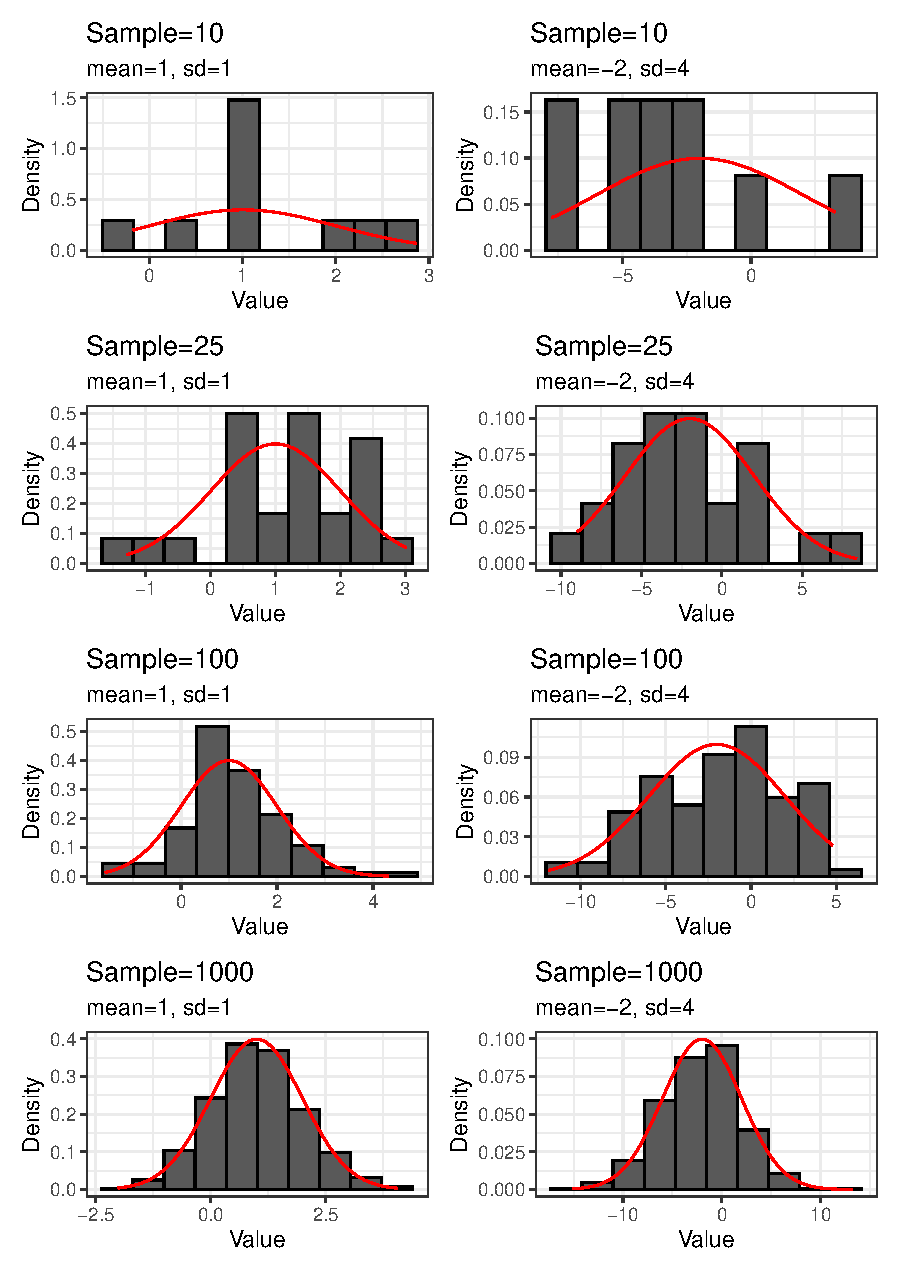
\includegraphics[width=\maxwidth]{figure/unnamed-chunk-5-1} 
\end{knitrout}
	\caption{Histograms of each set of data with superimposed true density function}
\label{plot3} %we can now reference plot1
\end{center}
\end{figure}
As we can see, the bigger sample we have, the closer the resulting histogram is to the real density function that we built on our set of parameters. We can notice that it's particularly true for $n>30$.\\
\begin{enumerate}
  \item Our PDF is such a good fit for the data because we are using \texttt{rnorm()} function that randomly generates numbers for the normal distribution. 
  \item A good fit can also be explained via Central Limit Theorem: as our sample enlarges, the distribution of our random variable follows a normal distribution.
\end{enumerate}
  
\end{enumerate}
%%%%%%%%%%%%%%%%%%%%%%%%%%%%%%%%%%%%%%%%%%%%%%%%%%%%%%%%%%%%%%%%%%%%%%%%%%%%%%%%%%%%%%%%%%%
%%%%%%%%%%%%%%%%%%%%%%%%%%%%%%%%%%%%%%%%%%%%%%%%%%%%%%%%%%%%%%%%%%%%%%%%%%%%%%%%%%%%%%%%%%%
%%%%%%%%%  Question 2
%%%%%%%%%%%%%%%%%%%%%%%%%%%%%%%%%%%%%%%%%%%%%%%%%%%%%%%%%%%%%%%%%%%%%%%%%%%%%%%%%%%%%%%%%%%
%%%%%%%%%%%%%%%%%%%%%%%%%%%%%%%%%%%%%%%%%%%%%%%%%%%%%%%%%%%%%%%%%%%%%%%%%%%%%%%%%%%%%%%%%%%
\item Continue with the continuous distribution you selected for Question \ref{Q1}.
\begin{enumerate}
  %%%%%%%%%%%%%%%%%%%%%%%%%%%%%%%%%%%%%%%%%%%%%%%%%%%%%%%%%%%%%%%%%%%%%%%%%%%%%%%%%%%%%%%%%%%
  %%%%%%%%%  Part (a)
  %%%%%%%%%%%%%%%%%%%%%%%%%%%%%%%%%%%%%%%%%%%%%%%%%%%%%%%%%%%%%%%%%%%%%%%%%%%%%%%%%%%%%%%%%%%
  \item Provide the mean, standard deviation, skewness, and kurtosis of the PDF.
  Ensure to interpret each.
  %%%%%%%%%%%%%%%%%%%%%%%%%%%%%%%%%%%%%%%%%%%%%%%%%%%%%%%%%%%%%%%%%%%%%%%%%%%%%%%%%%%%%%%%%%%
  %%%%%%%%%  Part (b)
  %%%%%%%%%%%%%%%%%%%%%%%%%%%%%%%%%%%%%%%%%%%%%%%%%%%%%%%%%%%%%%%%%%%%%%%%%%%%%%%%%%%%%%%%%%%
  \item Generate a random sample of size $n=10, 25, 100$, and $1000$ for your 
  two sets of parameter(s). Calculate the sample mean, standard deviation, 
  skewness, and kurtosis. Interpret the results.
  %%%%%%%%%%%%%%%%%%%%%%%%%%%%%%%%%%%%%%%%%%%%%%%%%%%%%%%%%%%%%%%%%%%%%%%%%%%%%%%%%%%%%%%%%%%
  %%%%%%%%%  Part (c)
  %%%%%%%%%%%%%%%%%%%%%%%%%%%%%%%%%%%%%%%%%%%%%%%%%%%%%%%%%%%%%%%%%%%%%%%%%%%%%%%%%%%%%%%%%%%
  \item Generate a random sample of size $n=10$ for your two sets of parameter(s).
  Calculate the method of moments estimator(s) and maximum likelihood estimator(s).
  In a $1 \times 2$ grid, plot a histogram of each set of data with (1) the method 
  of moments estimated distribution, (2) the maximum likelihood estimated 
  distribution, and superimpose the true distribution in both.
  %%%%%%%%%%%%%%%%%%%%%%%%%%%%%%%%%%%%%%%%%%%%%%%%%%%%%%%%%%%%%%%%%%%%%%%%%%%%%%%%%%%%%%%%%%%
  %%%%%%%%%  Part (d)
  %%%%%%%%%%%%%%%%%%%%%%%%%%%%%%%%%%%%%%%%%%%%%%%%%%%%%%%%%%%%%%%%%%%%%%%%%%%%%%%%%%%%%%%%%%%
  \item Generate a random sample of size $n=25$ for your two sets of parameter(s).
  Calculate the method of moments estimator(s) and maximum likelihood estimator(s). 
  In a $1 \times 2$ grid, plot a histogram of each set of data with (1) the method 
  of moments estimated distribution, (2) the maximum likelihood estimated distribution, 
  and superimpose the true distribution in both.
  %%%%%%%%%%%%%%%%%%%%%%%%%%%%%%%%%%%%%%%%%%%%%%%%%%%%%%%%%%%%%%%%%%%%%%%%%%%%%%%%%%%%%%%%%%%
  %%%%%%%%%  Part (e)
  %%%%%%%%%%%%%%%%%%%%%%%%%%%%%%%%%%%%%%%%%%%%%%%%%%%%%%%%%%%%%%%%%%%%%%%%%%%%%%%%%%%%%%%%%%%
  \item Generate a random sample of size $n=100$ for your two sets of parameter(s). 
  Calculate the method of moments estimator(s) and maximum likelihood estimator(s).
  In a $1 \times 2$ grid, plot a histogram of each set of data with (1) the method 
  of moments estimated distribution, (2) the maximum likelihood estimated distribution,
  and superimpose the true distribution in both.
  %%%%%%%%%%%%%%%%%%%%%%%%%%%%%%%%%%%%%%%%%%%%%%%%%%%%%%%%%%%%%%%%%%%%%%%%%%%%%%%%%%%%%%%%%%%
  %%%%%%%%%  Part (f)
  %%%%%%%%%%%%%%%%%%%%%%%%%%%%%%%%%%%%%%%%%%%%%%%%%%%%%%%%%%%%%%%%%%%%%%%%%%%%%%%%%%%%%%%%%%%
  \item Generate a random sample of size $n=100$ for your two sets of parameter(s). 
  Calculate the method of moments estimator(s) and maximum likelihood estimator(s). 
  In a $1 \times 2$ grid, plot a histogram of each set of data with (1) the method 
  of moments estimated distribution, (2) the maximum likelihood estimated distribution, 
  and superimpose the true distribution in both.
  %%%%%%%%%%%%%%%%%%%%%%%%%%%%%%%%%%%%%%%%%%%%%%%%%%%%%%%%%%%%%%%%%%%%%%%%%%%%%%%%%%%%%%%%%%%
  %%%%%%%%%  Part (g)
  %%%%%%%%%%%%%%%%%%%%%%%%%%%%%%%%%%%%%%%%%%%%%%%%%%%%%%%%%%%%%%%%%%%%%%%%%%%%%%%%%%%%%%%%%%%
  \item Comment on the results of parts (c)-(f). 
\end{enumerate}
\newpage
%%%%%%%%%%%%%%%%%%%%%%%%%%%%%%%%%%%%%%%%%%%%%%%%%%%%%%%%%%%%%%%%%%%%%%%%%%%%%%%%%%%%%%%%%%%
%%%%%%%%%%%%%%%%%%%%%%%%%%%%%%%%%%%%%%%%%%%%%%%%%%%%%%%%%%%%%%%%%%%%%%%%%%%%%%%%%%%%%%%%%%%
%%%%%%%%%  Question 3
%%%%%%%%%%%%%%%%%%%%%%%%%%%%%%%%%%%%%%%%%%%%%%%%%%%%%%%%%%%%%%%%%%%%%%%%%%%%%%%%%%%%%%%%%%%
%%%%%%%%%%%%%%%%%%%%%%%%%%%%%%%%%%%%%%%%%%%%%%%%%%%%%%%%%%%%%%%%%%%%%%%%%%%%%%%%%%%%%%%%%%%
  \item\label{Q3} Select a discrete distribution (not the Poisson). It does not 
  have to be one that we cover in the notes! To explore the PMF of your distribution, 
  specify two sets of parameter(s) for your distribution.
  \begin{enumerate}
  %%%%%%%%%%%%%%%%%%%%%%%%%%%%%%%%%%%%%%%%%%%%%%%%%%%%%%%%%%%%%%%%%%%%%%%%%%%%%%%%%%%%%%%%%%%
  %%%%%%%%%  Part (a)
  %%%%%%%%%%%%%%%%%%%%%%%%%%%%%%%%%%%%%%%%%%%%%%%%%%%%%%%%%%%%%%%%%%%%%%%%%%%%%%%%%%%%%%%%%%%
  \item \textbf{History} Discuss what types of random variables are modeled with 
  your distribution. Be sure to include a discussion about the support and ensure
  to provide the mass function, and CDF. This requires some internet research -- 
  what's the history of the distribution, why was it created and named? What are
  some exciting applications of this distribution? Cite all of your sources.\\
  
\textbf{Solution:}\\ The discrete distribution we have chosen is the Bernoulli distribution. The Bernoulli distribution  is a discrete probability distribution for a Bernoulli trial - a probabilistic experiment that can have one of two outcomes, success $\mathrm{(x = 1)}$ and failure $\mathrm{(x = 0)}$, and in which the probability fo success is $p$. Often $p$  is called the Bernoulli probability parameter \citep{forbes_stat}. In Bernoulli distribution, the random variable $X$ can have only one of two values: 0 or 1. This means that the support of our discrete random variable is the set $\mathrm{\{0,1\}}$. This distribution can be summarized as follows:
\begin{align*}
  p               &\in (0,1)                                                                               &\text{\textbf{[Parameter]}}\\
  \mathcal{X}     & = \{x: x \in \{0,1\}\}                                                                   &\text{\textbf{[Support]}}\\
  f_{X}(x \mid p) & = p^{x} (1-p)^{1-x}I(x \in \{0,1\})                                                      &\text{\textbf{[PMF]}}\\
  F_{X}(x \mid p) & = P(X \leq \left\lfloor x \right\rfloor)\\
                  & = [(1-p)I(\left\lfloor x \right\rfloor = 0)] + I(\left\lfloor x \right\rfloor \geq 1)  &\text{\textbf{[CDF]}}\\
\end{align*}
Simply, the Bernoulli distribution can be thought of as a model for the set of possible outcomes of any single experiment that asks a yes-no question \citep{bernoulli_brilliant}. This distribution is named after the 17th century Swiss mathematician Jacob Bernoulli, because he was the one who explicitly defined the concept of Bernoulli trial (in his book \emph{Ars Conjectandi}) described above. Bernoulli distribution serves as a building block for discrete distributions which model Bernoulli trials, such as Binomial distribution and geometric distribution \citep{prob_world}. Logistic regression, a widely used classification model that models a binary outcome, also takes advantage of the Bernoulli distribution \citep{logistic_regression}.

Since the Bernoulli distribution is not cataloged by R, we have to introduce it into our calculations with the  following functions:

\begin{knitrout}
\definecolor{shadecolor}{rgb}{0.969, 0.969, 0.969}\color{fgcolor}\begin{kframe}
\begin{alltt}
\hlcom{# Bernoulli PMF}
\hlstd{dbern}\hlkwb{<-}\hlkwa{function}\hlstd{(}\hlkwc{x}\hlstd{,}\hlkwc{prob}\hlstd{)\{}
  \hlkwa{if}\hlstd{(prob}\hlopt{<}\hlnum{0} \hlopt{|} \hlstd{prob}\hlopt{>}\hlnum{1}\hlstd{)\{}
    \hlstd{errormsg} \hlkwb{<-} \hlstr{"This function is only valid for success probabilities between 0 and 1."}
    \hlkwd{stop}\hlstd{(errormsg)}
  \hlstd{\}}
  \hlstd{indicator} \hlkwb{<-} \hlkwd{rep}\hlstd{(}\hlnum{0}\hlstd{,} \hlkwd{length}\hlstd{(x))}
  \hlstd{indicator[x}\hlopt{==}\hlnum{0}\hlstd{]} \hlkwb{<-} \hlnum{1} \hlcom{# indicator should be one if x=0}
  \hlstd{indicator[x}\hlopt{==}\hlnum{1}\hlstd{]} \hlkwb{<-} \hlnum{1} \hlcom{# indicator should be one if x=1}
  \hlstd{fx} \hlkwb{<-} \hlstd{(prob}\hlopt{^}\hlstd{x} \hlopt{*} \hlstd{(}\hlnum{1}\hlopt{-}\hlstd{prob)}\hlopt{^}\hlstd{(}\hlnum{1}\hlopt{-}\hlstd{x))} \hlopt{*} \hlstd{indicator} \hlcom{# PMF formula}
  \hlkwd{return}\hlstd{(fx)}
\hlstd{\}}
\hlcom{# Bernoulli CDF}
\hlstd{pbern}\hlkwb{<-}\hlkwa{function}\hlstd{(}\hlkwc{q}\hlstd{,} \hlkwc{prob}\hlstd{)\{}
  \hlkwa{if}\hlstd{(prob}\hlopt{<}\hlnum{0} \hlopt{|} \hlstd{prob}\hlopt{>}\hlnum{1}\hlstd{)\{}
    \hlstd{errormsg}\hlkwb{<-}\hlstr{"This function is only valid for success probabilities between 0 and 1."}
    \hlkwd{stop}\hlstd{(errormsg)}
  \hlstd{\}}
  \hlstd{indicator1} \hlkwb{<-} \hlkwd{rep}\hlstd{(}\hlnum{1}\hlstd{,} \hlkwd{length}\hlstd{(q))}
  \hlstd{indicator1[q} \hlopt{!=} \hlnum{0}\hlstd{]} \hlkwb{<-} \hlnum{0} \hlcom{#indicator should be zero if x!=0}
  \hlstd{indicator2} \hlkwb{<-} \hlkwd{rep}\hlstd{(}\hlnum{1}\hlstd{,} \hlkwd{length}\hlstd{(q))}
  \hlstd{indicator2[q} \hlopt{<} \hlnum{1}\hlstd{]} \hlkwb{<-} \hlnum{0} \hlcom{#indicator should be zero if x<1}
  \hlstd{Fx} \hlkwb{<-} \hlstd{(}\hlnum{1}\hlopt{-}\hlstd{prob)} \hlopt{*} \hlstd{indicator1} \hlopt{+} \hlstd{indicator2}
  \hlkwd{return}\hlstd{(Fx)}
\hlstd{\}}
\end{alltt}
\end{kframe}
\end{knitrout}
The R packages Tidyverse \citep{tidyverse} and Patchwork \citep{Patchwork} will be used in all of the following plots in question 3.
  %%%%%%%%%%%%%%%%%%%%%%%%%%%%%%%%%%%%%%%%%%%%%%%%%%%%%%%%%%%%%%%%%%%%%%%%%%%%%%%%%%%%%%%%%%%
  %%%%%%%%%  Part (b)
  %%%%%%%%%%%%%%%%%%%%%%%%%%%%%%%%%%%%%%%%%%%%%%%%%%%%%%%%%%%%%%%%%%%%%%%%%%%%%%%%%%%%%%%%%%%
	\item Show that you have a valid PMF. You can show this approximately by 
	calculating the series in a repeat loop until probability mass evaluations are 
	infinitesimally small.
	
	\textbf{Solution:} For a PMF to be valid, it has to fulfill the following statements:
	\begin{enumerate}
	\item[1.] $0 \leq f_{X}(x) \leq 1$ for all $x \in \mathbb{R}$
	\item[2.] $ \sum_{-\infty}^{\infty} f_{X} = \sum_{\mathcal{X}}f_{X} = 1$
	\end{enumerate}
	
	By definition, the Bernoulli distribution satisfies statement 1, since the support is {0,1} and the probability parameter $\mathrm{p \in (0,1)}$, so the term for PMF (see above) cannot have a value smaller than 0 or greater than 1.
	
	We can also show that the statement 2 is true for the Bernoulli distribution:
	
	\begin{align*}
	  \sum_{\mathcal{X}}f_{X} = \sum_{x = 0}^{1}f_{X}(x) &= \sum_{x = 0}^{1}p^{x}(1-p)^{1-x}\\
	  &= p^{0}(1-p)^{1-0} +p^{1}(1-p)^{1-1}\\
	  &= (1)(1-p) + p(1)\\
	  &= 1-p+p\\
	  &= 1
	\end{align*}
	
	Therefore, we have a valid PMF for our distribution.
	
	%%%%%%%%%%%%%%%%%%%%%%%%%%%%%%%%%%%%%%%%%%%%%%%%%%%%%%%%%%%%%%%%%%%%%%%%%%%%%%%%%%%%%%%%%%%
  %%%%%%%%%  Part (c)
  %%%%%%%%%%%%%%%%%%%%%%%%%%%%%%%%%%%%%%%%%%%%%%%%%%%%%%%%%%%%%%%%%%%%%%%%%%%%%%%%%%%%%%%%%%%
	\item Find the median for your two sets of parameter(s). Conduct some research 
	to find the median based on our PMF to confirm that your numerical approach is
	correct.\\ 
	
	\textbf{Solution:} In the Bernoulli distribution, where p is the probability parameter and $\mathrm{q = 1 - p}$, when p\textgreater q, there are more "successes" (that is when $X$ is 1) than failure (when $X$ is 0), so the median must also be a success. Similar, when q\textgreater p, there are more "failures" than "successes", hence resulting in the median being 0. When $\mathrm{p = q}$, there is an equal probability of $X$ being 0 or 1, thus the median is ambiguous. Therefore, the median for when $\mathrm{p = 0.4}$ is zero and the median for when $\mathrm{p = 0.6}$ is 1. Further inquiry \textbf{(QUOTE: Wikipedia)} suggests that this really is the case for the median of the Bernoulli distribution:\
	\begin{align*}
	Median=\begin{cases}
          0 \quad &\text{if} \, p < 1/2\\
          [0,1] \quad &\text{if} \, p = 1/2\\
          1 \quad &\text{if} \, p > 1/2\\
     \end{cases}
	\end{align*}
	%%%%%%%%%%%%%%%%%%%%%%%%%%%%%%%%%%%%%%%%%%%%%%%%%%%%%%%%%%%%%%%%%%%%%%%%%%%%%%%%%%%%%%%%%%%
  %%%%%%%%%  Part (d)
  %%%%%%%%%%%%%%%%%%%%%%%%%%%%%%%%%%%%%%%%%%%%%%%%%%%%%%%%%%%%%%%%%%%%%%%%%%%%%%%%%%%%%%%%%%%
	\item \label{q3PMF} Graph the PMF for several values of the parameter(s) 
	including the two sets you specified. What does changing the parameter(s) do 
	to the shape of the PMF?
	
	\textbf{Solution:} We can plot the PMF of the Bernoulli distribution for different parameters.Note that the initially chosen parameters were $\mathrm{p =0.4}$ and $\mathrm{p=0.6}$. Let us also look at the PMF when the parameter values are 0.5, and 0.8.
	
\begin{knitrout}
\definecolor{shadecolor}{rgb}{0.969, 0.969, 0.969}\color{fgcolor}\begin{kframe}
\begin{alltt}
\hlkwd{library}\hlstd{(tidyverse)}
\hlkwd{library}\hlstd{(patchwork)}
\hlstd{plotbernPMF} \hlkwb{<-} \hlkwa{function}\hlstd{(}\hlkwc{prob}\hlstd{)\{} \hlcom{# Pass in the success probability}
  \hlstd{ggdat} \hlkwb{<-} \hlkwd{data.frame}\hlstd{(}\hlkwc{x} \hlstd{= (}\hlopt{-}\hlnum{1}\hlopt{:}\hlnum{2}\hlstd{),}
                      \hlkwc{f} \hlstd{=} \hlkwd{dbern}\hlstd{(}\hlkwc{x} \hlstd{= (}\hlopt{-}\hlnum{1}\hlopt{:}\hlnum{2}\hlstd{),} \hlkwc{prob} \hlstd{= prob),}
                      \hlkwc{F} \hlstd{=} \hlkwd{pbern}\hlstd{(}\hlkwc{q} \hlstd{= (}\hlopt{-}\hlnum{1}\hlopt{:}\hlnum{2}\hlstd{),} \hlkwc{prob} \hlstd{= prob))}
  \hlcom{## Plot PMF}
  \hlstd{PMF} \hlkwb{<-} \hlkwd{ggplot}\hlstd{(}\hlkwc{data} \hlstd{= ggdat,} \hlkwd{aes}\hlstd{(}\hlkwc{x} \hlstd{= x))} \hlopt{+}
    \hlkwd{geom_linerange}\hlstd{(}\hlkwd{aes}\hlstd{(}\hlkwc{ymax} \hlstd{= f),} \hlkwc{ymin} \hlstd{=} \hlnum{0}\hlstd{)} \hlopt{+}
    \hlkwd{geom_hline}\hlstd{(}\hlkwc{yintercept} \hlstd{=} \hlnum{0}\hlstd{)} \hlopt{+}
    \hlkwd{theme_bw}\hlstd{()} \hlopt{+}
    \hlkwd{ylim}\hlstd{(}\hlnum{0}\hlstd{,} \hlnum{1}\hlstd{)} \hlopt{+}
    \hlkwd{xlab}\hlstd{(}\hlstr{"X"}\hlstd{)} \hlopt{+}
    \hlkwd{ylab}\hlstd{(}\hlkwd{bquote}\hlstd{(f[x](x)))} \hlopt{+}
    \hlkwd{ggtitle}\hlstd{(}\hlstr{"Bernoulli Distribution"}\hlstd{,}\hlkwc{subtitle} \hlstd{=} \hlkwd{paste}\hlstd{(}\hlstr{"p ="}\hlstd{, prob))}

  \hlkwd{return}\hlstd{(PMF)}
\hlstd{\}}

\hlkwd{plotbernPMF}\hlstd{(}\hlnum{0.4}\hlstd{)} \hlopt{+} \hlkwd{plotbernPMF}\hlstd{(}\hlnum{0.5}\hlstd{)} \hlopt{+} \hlkwd{plotbernPMF}\hlstd{(}\hlnum{0.6}\hlstd{)} \hlopt{+} \hlkwd{plotbernPMF}\hlstd{(}\hlnum{0.8}\hlstd{)}
\end{alltt}
\end{kframe}
\end{knitrout}

\begin{figure}[H]
  \begin{center}
  % This code is evaluated, but not printed
  % note below I use message=FALSE and warning=FALSE to surpress what's printed
  % when running library(ggmap) or library(patchwork) which would otherwise cause
  % an error because Sweave is expecting just a graph (not a graph + text)
\begin{knitrout}
\definecolor{shadecolor}{rgb}{0.969, 0.969, 0.969}\color{fgcolor}
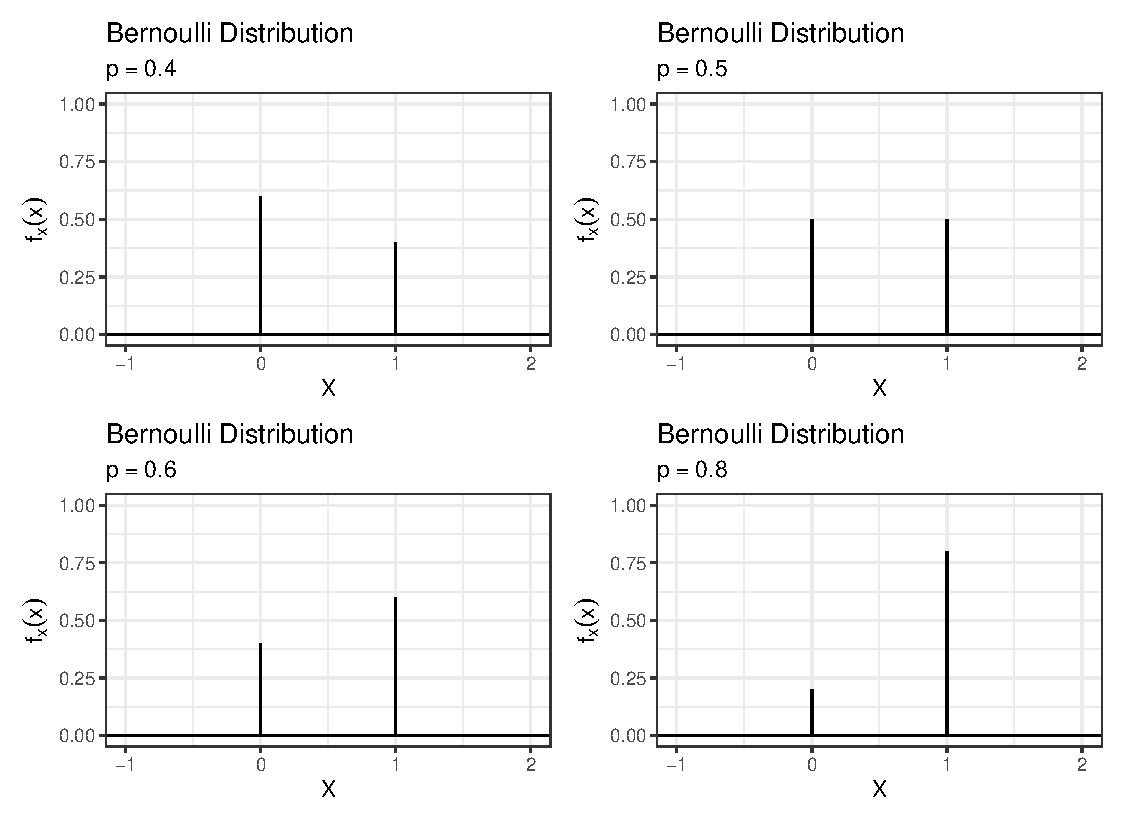
\includegraphics[width=\maxwidth]{figure/unnamed-chunk-7-1} 
\end{knitrout}
    \caption{The CDF of the Bernoulli distribution for different probability parameters p}
    \label{P3fig_1} %we can now reference P3fig_1
  \end{center}
\end{figure}

We observe the same characteristic of the Bernoulli distribution in Figure \ref{P3fig_1} as we discussed about its median above. If the $\mathrm{p<0.5}$ then there are more failures than successes, indicated by the taller PMF at 0. On the other hand, if If the $\mathrm{p>0.5}$ then there are more successes than failures, which is reflected in the PMF plot being taller at 1. The plot of the PMF when $\mathrm{p=0.5}$ suggests that there is an equal chance for success as there is for failure.
  %%%%%%%%%%%%%%%%%%%%%%%%%%%%%%%%%%%%%%%%%%%%%%%%%%%%%%%%%%%%%%%%%%%%%%%%%%%%%%%%%%%%%%%%%%%
  %%%%%%%%%  Part (e)
  %%%%%%%%%%%%%%%%%%%%%%%%%%%%%%%%%%%%%%%%%%%%%%%%%%%%%%%%%%%%%%%%%%%%%%%%%%%%%%%%%%%%%%%%%%%
	 \item Graph the CDF for the same values of the parameter(s) as you did in 
	 Question \ref{q3PMF}. What does changing the parameter(s) do to the shape of 
	 the CDF? Comment on the aspects of the CDFs that show that the CDF is valid.
	 
	 \textbf{Solution:} We can plot the CDF of the Bernoulli distribution for the different parameters 0.4, 0.5, 0.6, and 0.8 below:
\begin{knitrout}
\definecolor{shadecolor}{rgb}{0.969, 0.969, 0.969}\color{fgcolor}\begin{kframe}
\begin{alltt}
\hlstd{plotbernCDF} \hlkwb{<-} \hlkwa{function}\hlstd{(}\hlkwc{prob}\hlstd{)\{} \hlcom{# Pass in the success probability}
  \hlstd{ggdat} \hlkwb{<-} \hlkwd{data.frame}\hlstd{(}\hlkwc{x} \hlstd{= (}\hlopt{-}\hlnum{1}\hlopt{:}\hlnum{2}\hlstd{),}
                      \hlkwc{f} \hlstd{=} \hlkwd{dbern}\hlstd{(}\hlkwc{x} \hlstd{= (}\hlopt{-}\hlnum{1}\hlopt{:}\hlnum{2}\hlstd{),} \hlkwc{prob} \hlstd{= prob),}
                      \hlkwc{F} \hlstd{=} \hlkwd{pbern}\hlstd{(}\hlkwc{q} \hlstd{= (}\hlopt{-}\hlnum{1}\hlopt{:}\hlnum{2}\hlstd{),} \hlkwc{prob} \hlstd{= prob))}
  \hlstd{ggdat.openpoints} \hlkwb{<-} \hlkwd{data.frame}\hlstd{(}\hlkwc{x} \hlstd{= ggdat}\hlopt{$}\hlstd{x,}
                                 \hlkwc{y} \hlstd{=} \hlkwd{pbern}\hlstd{(ggdat}\hlopt{$}\hlstd{x}\hlopt{-}\hlnum{1}\hlstd{,} \hlkwc{prob} \hlstd{= prob))}
  \hlstd{ggdat.closedpoints} \hlkwb{<-} \hlkwd{data.frame}\hlstd{(}\hlkwc{x} \hlstd{= ggdat}\hlopt{$}\hlstd{x,}
                                   \hlkwc{y} \hlstd{=} \hlkwd{pbern}\hlstd{(ggdat}\hlopt{$}\hlstd{x,}\hlkwc{prob}\hlstd{=prob))}
  \hlstd{CDF}\hlkwb{<-}\hlkwd{ggplot}\hlstd{(}\hlkwc{data} \hlstd{= ggdat,} \hlkwd{aes}\hlstd{(}\hlkwc{x} \hlstd{= x,} \hlkwc{y} \hlstd{= F))} \hlopt{+}
    \hlkwd{geom_step}\hlstd{()}\hlopt{+}
    \hlkwd{geom_point}\hlstd{(}\hlkwc{data} \hlstd{= ggdat.openpoints,} \hlkwd{aes}\hlstd{(}\hlkwc{x} \hlstd{= x,} \hlkwc{y} \hlstd{= y),} \hlkwc{shape} \hlstd{=} \hlnum{1}\hlstd{)} \hlopt{+}
    \hlkwd{geom_point}\hlstd{(}\hlkwc{data} \hlstd{= ggdat.closedpoints,} \hlkwd{aes}\hlstd{(}\hlkwc{x} \hlstd{= x,} \hlkwc{y} \hlstd{= y))} \hlopt{+}
    \hlkwd{geom_hline}\hlstd{(}\hlkwc{yintercept} \hlstd{=} \hlnum{0.5}\hlstd{,} \hlkwc{linetype}\hlstd{=}\hlstr{"dotted"}\hlstd{,} \hlkwc{color}\hlstd{=}\hlstr{"red"}\hlstd{)}\hlopt{+}
    \hlkwd{theme_bw}\hlstd{()}\hlopt{+}
    \hlkwd{xlab}\hlstd{(}\hlstr{"X"}\hlstd{)}\hlopt{+}
    \hlkwd{ylab}\hlstd{(}\hlkwd{bquote}\hlstd{(F[x](x)))}\hlopt{+}
    \hlkwd{ggtitle}\hlstd{(}\hlstr{"Bernoulli CDF"}\hlstd{,}\hlkwc{subtitle}\hlstd{=(}\hlkwd{paste}\hlstd{(}\hlstr{"p ="}\hlstd{, prob)))}
  \hlkwd{return}\hlstd{(CDF)}
\hlstd{\}}
\hlkwd{plotbernCDF}\hlstd{(}\hlnum{0.4}\hlstd{)} \hlopt{+} \hlkwd{plotbernCDF}\hlstd{(}\hlnum{0.5}\hlstd{)} \hlopt{+} \hlkwd{plotbernCDF}\hlstd{(}\hlnum{0.6}\hlstd{)} \hlopt{+} \hlkwd{plotbernCDF}\hlstd{(}\hlnum{0.8}\hlstd{)}
\end{alltt}
\end{kframe}
\end{knitrout}
\begin{figure}[H]
  \begin{center}
  % This code is evaluated, but not printed
  % note below I use message=FALSE and warning=FALSE to surpress what's printed
  % when running library(ggmap) or library(patchwork) which would otherwise cause
  % an error because Sweave is expecting just a graph (not a graph + text)
\begin{knitrout}
\definecolor{shadecolor}{rgb}{0.969, 0.969, 0.969}\color{fgcolor}
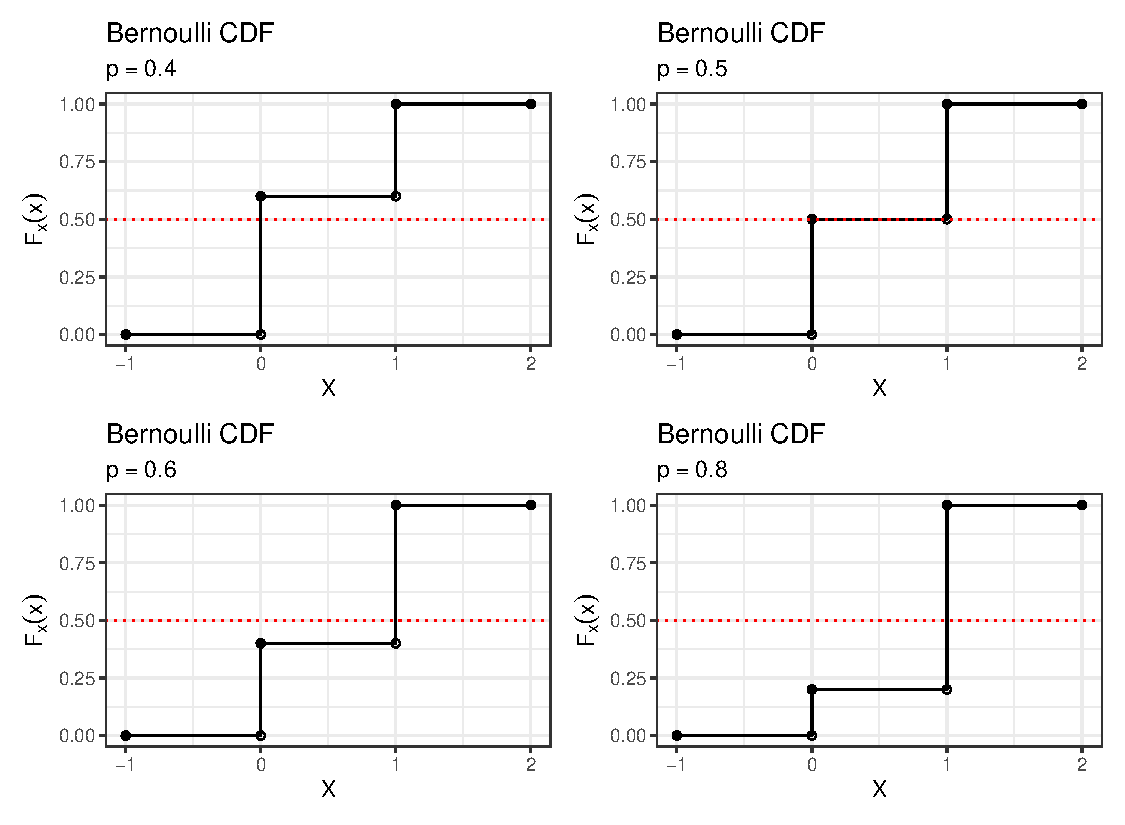
\includegraphics[width=\maxwidth]{figure/unnamed-chunk-8-1} 
\end{knitrout}
    \caption{The CDF of the Bernoulli distribution for different probability parameters p}
    \label{P3fig_2} %we can now reference P3fig_1
  \end{center}
\end{figure}

In the Figure \ref{P3fig_2}, we can see that with increasing p, the most of the "area" under the CDF is moving towards 1, which correctly indicates that the number of successes increase as the value of p increases. Furthermore, we can see that in all the CDF plots, the functions always add up to 1. The CDF are also monotonically increasing towards the right. All of these above characteristics together indicate that our CDF is valid. Notice that in all of the plots of Figure \ref{P3fig_2}, we have drawn a horizontal line at 1/2. This is another way we can determine the median of the Bernoulli distribution using the CDF. Where the horizontal line intersects the CDF indicates where the median is for the given value of p. These results agree with our results from problem 3(c).
	%%%%%%%%%%%%%%%%%%%%%%%%%%%%%%%%%%%%%%%%%%%%%%%%%%%%%%%%%%%%%%%%%%%%%%%%%%%%%%%%%%%%%%%%%%%
  %%%%%%%%%  Part (f)
  %%%%%%%%%%%%%%%%%%%%%%%%%%%%%%%%%%%%%%%%%%%%%%%%%%%%%%%%%%%%%%%%%%%%%%%%%%%%%%%%%%%%%%%%%%%
  \item Generate a random sample of size $n=10, 25, 100$, and $1000$ for your 
  two sets of parameter(s). In a $4 \times 2$ grid, plot a histogram (with bin 
  size 1) of each set of data and superimpose the true mass function at the 
  specified parameter values. Interpret the results.
  

  \textbf{Solution:} The two parameters we are working with are $\mathrm{p=0.4}$ and $\mathrm{p=0.6}$
\begin{knitrout}
\definecolor{shadecolor}{rgb}{0.969, 0.969, 0.969}\color{fgcolor}\begin{kframe}
\begin{alltt}
\hlcom{# Using sampling with replacement to generate arrays of 0 and 1}

\hlkwd{library}(tidyverse)
\hlkwd{library}(patchwork)

plot_df <- \hlkwd{list}( x1 = \hlkwd{bern_sample}(10, 0.4),
                 x2 = \hlkwd{bern_sample}(25, 0.4),
                 x3 = \hlkwd{bern_sample}(100, 0.4),
                 x4 = \hlkwd{bern_sample}(1000, 0.4),
                 y1 = \hlkwd{bern_sample}(10, 0.6),
                 y2 = \hlkwd{bern_sample}(25, 0.6),
                 y3 = \hlkwd{bern_sample}(100, 0.6),
                 y4 = \hlkwd{bern_sample}(1000, 0.6))

                 
buildingPlot2 <- \hlkwd{function}(source, prob, sample_size)\{
	  df <- \hlkwd{data.frame}(value=source) \hlcom{#turning values from the list into a df}
	  \hlkwd{colnames}(df) <- \hlstr{"value"} #changing the name of the column
	  df_PMF <- \hlkwd{data.frame}(x = (-1:2),
                      f = \hlkwd{dbern}(x = (-1:2), prob = prob))
	  answer<-\hlkwd{ggplot}(df, \hlkwd{aes}(value))+
	     \hlkwd{geom_histogram}(data = df, \hlkwd{aes}(y=..density..), binwidth=1,
	                 color=\hlstr{"black"})+
	  \hlkwd{geom_linerange}(data=df_PMF, \hlkwd{aes}(x=x, ymax = f), ymin = 0, size=2, color=\hlstr{"red"})+
	  \hlkwd{theme_bw}() +
	  \hlkwd{ggtitle}(\hlstr{"Bernoulli Distribution"},subtitle = \hlkwd{paste}(\hlstr{"Sample Size ="}, sample size, \hlstr{", Prob ="}, prob))
	  answer
	\}

x1 <- \hlkwd{buildingPlot2}(plot_df[1], 0.4, 10)
x2 <- \hlkwd{buildingPlot2}(plot_df[2], 0.4, 25)
x3 <- \hlkwd{buildingPlot2}(plot_df[3], 0.4, 100)
x4 <- \hlkwd{buildingPlot2}(plot_df[4], 0.4, 1000)

y1 <- \hlkwd{buildingPlot2}(plot_df[5], 0.6, 10)
y2 <- \hlkwd{buildingPlot2}(plot_df[6], 0.6, 25)
y3 <- \hlkwd{buildingPlot2}(plot_df[7], 0.6, 100)
y4 <- \hlkwd{buildingPlot2}(plot_df[8], 0.6, 1000)
		

(x1+y1)/(x2+y2)/(x3+y3)/(x4+y4)
\end{alltt}
\end{kframe}
\end{knitrout}

\begin{figure}[H]
  \begin{center}
  % This code is evaluated, but not printed
  % note below I use message=FALSE and warning=FALSE to surpress what's printed
  % when running library(ggmap) or library(patchwork) which would otherwise cause
  % an error because Sweave is expecting just a graph (not a graph + text)
  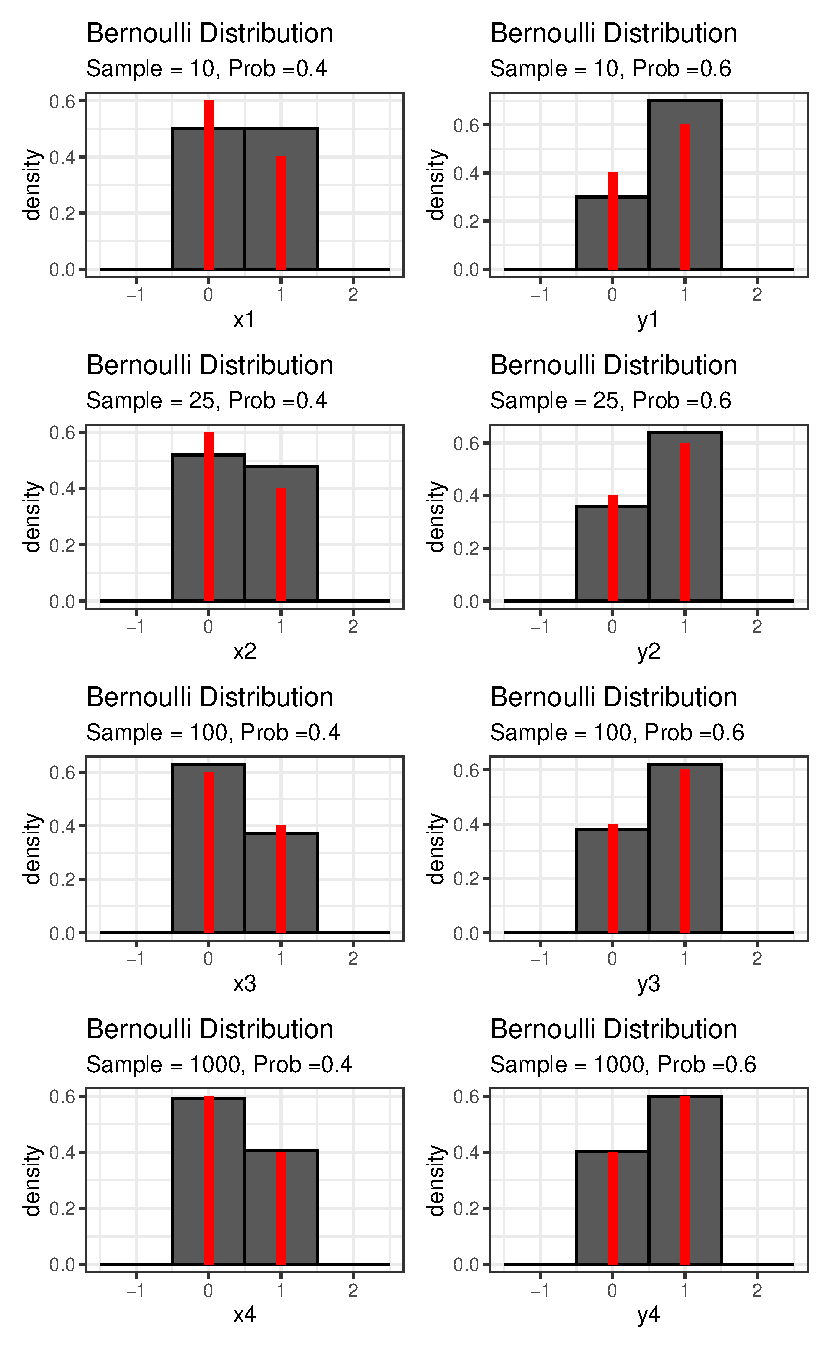
\includegraphics[width=5in, height=8.5in]{figure/histogram.pdf}
    \caption{(Top row) Samples of 10, 25, 100, 1000 for the Bernoulli distribution with p = 0.4. (Bottom row) Samples of 10, 25, 100, 1000 for the Bernoulli distribution with p = 0.6. In each plot the red lines indicate the true PMF function of the corresponding Bernoulli distribution. Notice that the y-axis indicates the prportional frequency in the histograms}
    \label{P3fig_3} %we can now reference P3fig_1
  \end{center}
\end{figure}
	\end{enumerate}
	For each of the cases of p (see the first and the second row of plots in Figure \ref{P3fig_3}), the more we sample, the better our histograms agree with the the true PMF of the Bernoulli distribution. These histograms above represent only one variation of the random sampling done on the Bernoulli distribution. While the histograms for n=1000 does not stray much from the PMF as we take newere samples, the smaller samples (10, 25) vary significantly from the PMF. From sample to sample, the results of the histograms vary (in terms of agreement with the true PMF). The larger the size of the sample, the more consistent is its agreement with the true PMF. 
	
%%%%%%%%%%%%%%%%%%%%%%%%%%%%%%%%%%%%%%%%%%%%%%%%%%%%%%%%%%%%%%%%%%%%%%%%%%%%%%%%%%%%%%%%%%%
%%%%%%%%%%%%%%%%%%%%%%%%%%%%%%%%%%%%%%%%%%%%%%%%%%%%%%%%%%%%%%%%%%%%%%%%%%%%%%%%%%%%%%%%%%%
%%%%%%%%%  Question 2
%%%%%%%%%%%%%%%%%%%%%%%%%%%%%%%%%%%%%%%%%%%%%%%%%%%%%%%%%%%%%%%%%%%%%%%%%%%%%%%%%%%%%%%%%%%
%%%%%%%%%%%%%%%%%%%%%%%%%%%%%%%%%%%%%%%%%%%%%%%%%%%%%%%%%%%%%%%%%%%%%%%%%%%%%%%%%%%%%%%%%%%
\item Continue with the discrete distribution you selected for Question \ref{Q3}.
\begin{enumerate}
  %%%%%%%%%%%%%%%%%%%%%%%%%%%%%%%%%%%%%%%%%%%%%%%%%%%%%%%%%%%%%%%%%%%%%%%%%%%%%%%%%%%%%%%%%%%
  %%%%%%%%%  Part (a)
  %%%%%%%%%%%%%%%%%%%%%%%%%%%%%%%%%%%%%%%%%%%%%%%%%%%%%%%%%%%%%%%%%%%%%%%%%%%%%%%%%%%%%%%%%%%
  \item Provide the mean, standard deviation, skewness, and kurtosis of the PMF. 
  Ensure to interpret each.
  %%%%%%%%%%%%%%%%%%%%%%%%%%%%%%%%%%%%%%%%%%%%%%%%%%%%%%%%%%%%%%%%%%%%%%%%%%%%%%%%%%%%%%%%%%%
  %%%%%%%%%  Part (b)
  %%%%%%%%%%%%%%%%%%%%%%%%%%%%%%%%%%%%%%%%%%%%%%%%%%%%%%%%%%%%%%%%%%%%%%%%%%%%%%%%%%%%%%%%%%%
  \item Generate a random sample of size $n=10, 25, 100$, and $1000$ for your 
  two sets of parameter(s). Calculate the sample mean, standard deviation, 
  skewness, and kurtosis. Interpret the results.
  %%%%%%%%%%%%%%%%%%%%%%%%%%%%%%%%%%%%%%%%%%%%%%%%%%%%%%%%%%%%%%%%%%%%%%%%%%%%%%%%%%%%%%%%%%%
  %%%%%%%%%  Part (c)
  %%%%%%%%%%%%%%%%%%%%%%%%%%%%%%%%%%%%%%%%%%%%%%%%%%%%%%%%%%%%%%%%%%%%%%%%%%%%%%%%%%%%%%%%%%%
  \item Generate a random sample of size $n=10$ for your two sets of parameter(s).
  Calculate the method of moments estimator(s) and maximum likelihood estimator(s).
  In a $1 \times 2$ grid, plot a histogram (with bin size 1) of each set of data 
  with (1) the method of moments estimated distribution, (2) the maximum likelihood 
  estimated distribution, and superimpose the true distribution in both.
  %%%%%%%%%%%%%%%%%%%%%%%%%%%%%%%%%%%%%%%%%%%%%%%%%%%%%%%%%%%%%%%%%%%%%%%%%%%%%%%%%%%%%%%%%%%
  %%%%%%%%%  Part (d)
  %%%%%%%%%%%%%%%%%%%%%%%%%%%%%%%%%%%%%%%%%%%%%%%%%%%%%%%%%%%%%%%%%%%%%%%%%%%%%%%%%%%%%%%%%%%
  \item Generate a random sample of size $n=25$ for your two sets of parameter(s). 
  Calculate the method of moments estimator(s) and maximum likelihood estimator(s).
  In a $1 \times 2$ grid, plot a histogram (with bin size 1) of each set of data 
  with (1) the method of moments estimated distribution, (2) the maximum likelihood 
  estimated distribution, and superimpose the true distribution in both.
  %%%%%%%%%%%%%%%%%%%%%%%%%%%%%%%%%%%%%%%%%%%%%%%%%%%%%%%%%%%%%%%%%%%%%%%%%%%%%%%%%%%%%%%%%%%
  %%%%%%%%%  Part (e)
  %%%%%%%%%%%%%%%%%%%%%%%%%%%%%%%%%%%%%%%%%%%%%%%%%%%%%%%%%%%%%%%%%%%%%%%%%%%%%%%%%%%%%%%%%%%
  \item Generate a random sample of size $n=100$ for your two sets of parameter(s).
  Calculate the method of moments estimator(s) and maximum likelihood estimator(s). 
  In a $1 \times 2$ grid, plot a histogram (with bin size 1) of each set of data 
  with (1) the method of moments estimated distribution, (2) the maximum likelihood
  estimated distribution, and superimpose the true distribution in both.
  %%%%%%%%%%%%%%%%%%%%%%%%%%%%%%%%%%%%%%%%%%%%%%%%%%%%%%%%%%%%%%%%%%%%%%%%%%%%%%%%%%%%%%%%%%%
  %%%%%%%%%  Part (f)
  %%%%%%%%%%%%%%%%%%%%%%%%%%%%%%%%%%%%%%%%%%%%%%%%%%%%%%%%%%%%%%%%%%%%%%%%%%%%%%%%%%%%%%%%%%%
  \item Generate a random sample of size $n=100$ for your two sets of parameter(s).
  Calculate the method of moments estimator(s) and maximum likelihood estimator(s).
  In a $1 \times 2$ grid, plot a histogram (with bin size 1) of each set of data 
  with (1) the method of moments estimated distribution, (2) the maximum likelihood
  estimated distribution, and superimpose the true distribution in both.
  %%%%%%%%%%%%%%%%%%%%%%%%%%%%%%%%%%%%%%%%%%%%%%%%%%%%%%%%%%%%%%%%%%%%%%%%%%%%%%%%%%%%%%%%%%%
  %%%%%%%%%  Part (g)
  %%%%%%%%%%%%%%%%%%%%%%%%%%%%%%%%%%%%%%%%%%%%%%%%%%%%%%%%%%%%%%%%%%%%%%%%%%%%%%%%%%%%%%%%%%%
  \item Comment on the results of parts (c)-(f). 
\end{enumerate}
\end{enumerate}%End overall enumerate
\newpage
\bibliography{bib}
\end{document}
